\documentclass[graphics]{beamer}

\usepackage{graphicx}
\usepackage{verbatim}
\usepackage{wrapfig}
\useoutertheme{shadow}
%\usecolortheme{orchid}
\usecolortheme{seahorse}


% math commands
\newcommand{\be}{\begin{eqnarray}}
\newcommand{\ee}{\end{eqnarray}}
\newcommand{\beq}{\begin{equation}}
\newcommand{\eeq}{\end{equation}}
\def\simless{\mathbin{\lower 3pt\hbox
      {$\rlap{\raise 5pt\hbox{$\char'074$}}\mathchar"7218$}}}
\def\simgreat{\mathbin{\lower 3pt\hbox
      {$\rlap{\raise 5pt\hbox{$\char'076$}}\mathchar"7218$}}} %> or of order

% variables

\def\toonscale{0.45}
\def\mboxy#1{\mbox{\small #1}}


\begin{comment}
\AtBeginSection[]{
  \frame{
    \frametitle{Outline}
    \tableofcontents[currentsection]
  }
}
\end{comment}

\title{Astrophysical measures of space and time
}
\subtitle{}
\author[U. Pen]{Ue-Li Pen
\\[8mm] 
}
\date{Sept 4, 2019}


\begin{document}


\begin{comment}
  \subsection{Outline}

  \frame{
    \frametitle{Outline}
    \tableofcontents
  }
\end{comment}

  \frame{
\vspace{-0.5in}
    \frametitle{Tools}
    \begin{itemize}
        \item Fast Radio Bursts and pulsars: use as high intensity light
          sources (highest known brightness temperatures in the
          universe) and as clocks 
        \item lensed by gravity and plasma
        \item use for gravitational wave detection, testing classical
          gravity, quantum gravity
        \item virtual lab: HPC computers (60,000+ cores at SciNet)
          \item celestial lab:  Algonquin Radio Telescope, VLBI, CHIME
    \end{itemize}
  }

  \frame{
    \frametitle{Research Environment}
    \begin{itemize}
      \item close collaborations with dynamic group of postdocs at
        CITA
      \item learn and build tools in astrophysical theory,
        computation, radio data
      \item work at field sites including Algonquin (Ontario), Penticton (BC).
    \end{itemize}
\vspace{-0.12in}\hspace{-.2in}
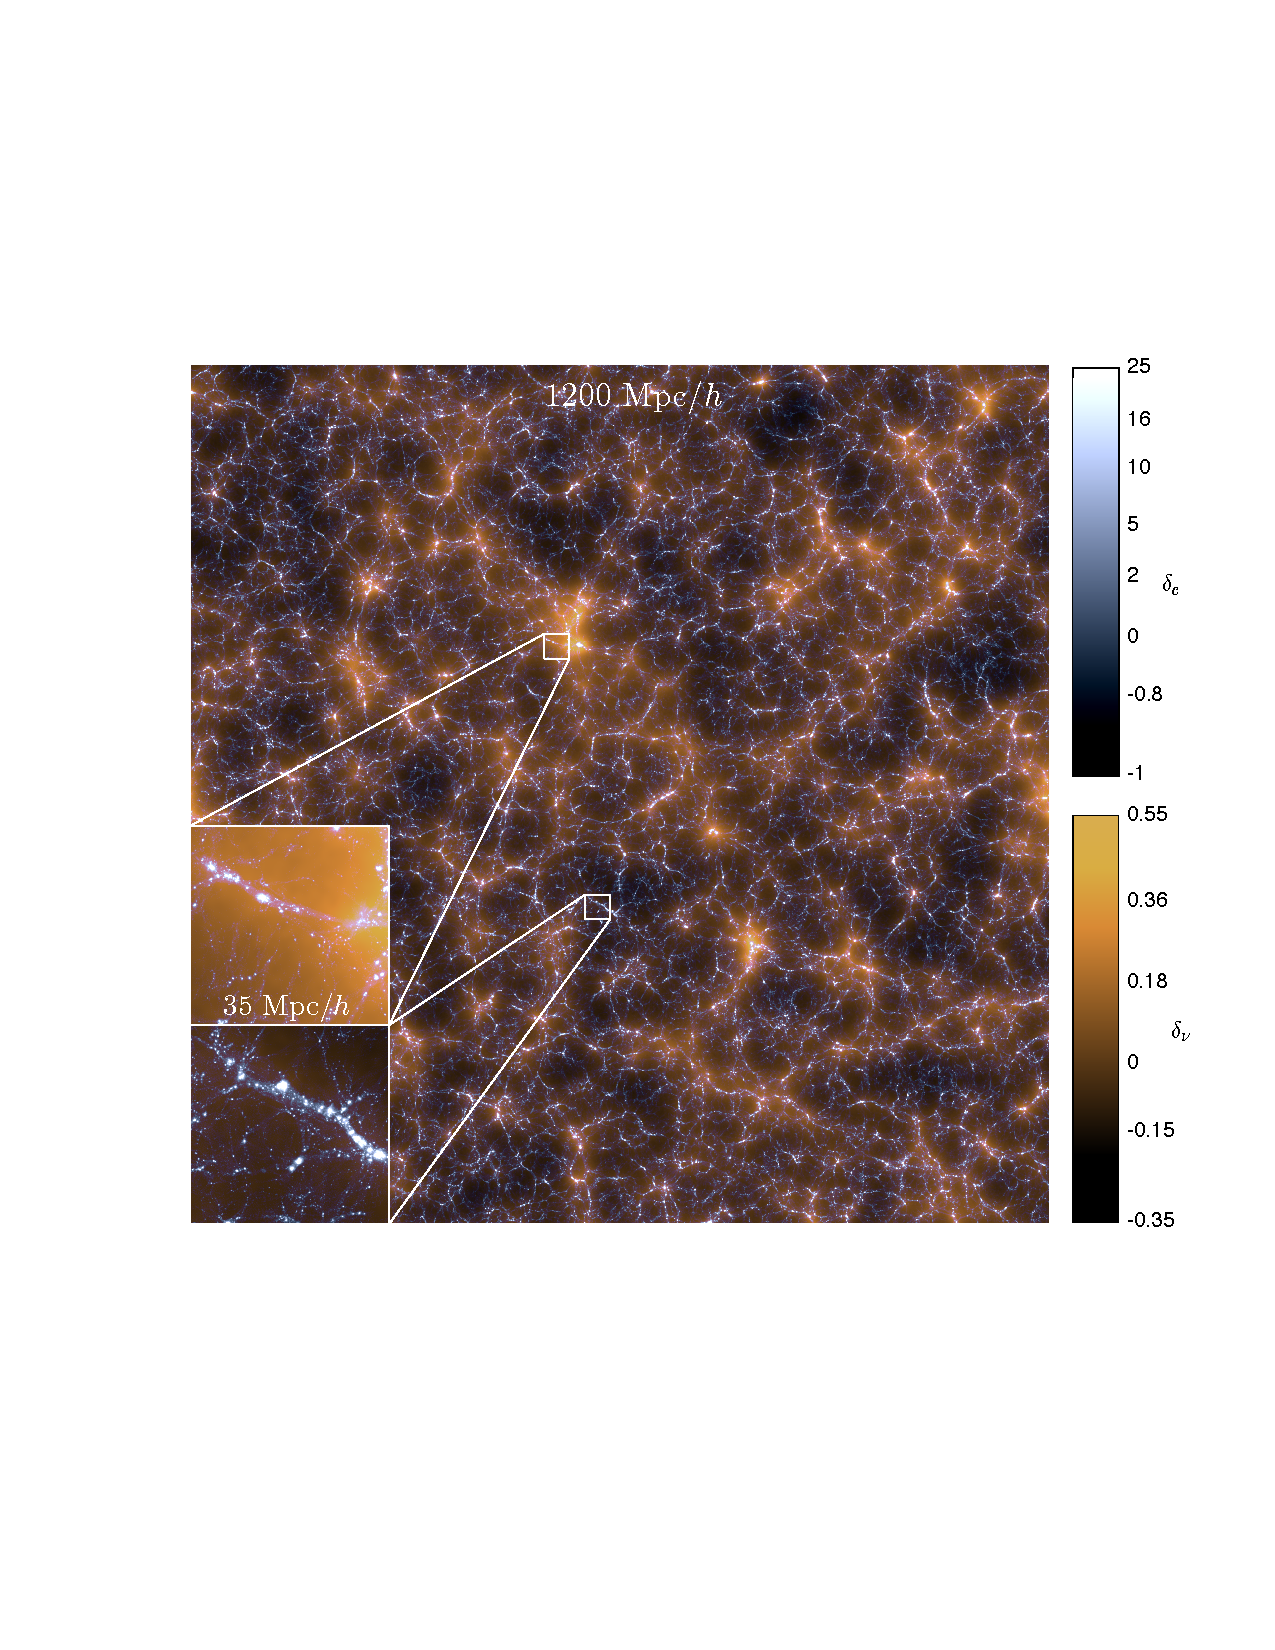
\includegraphics[width=2.3in]{Figures/tiannu.pdf}
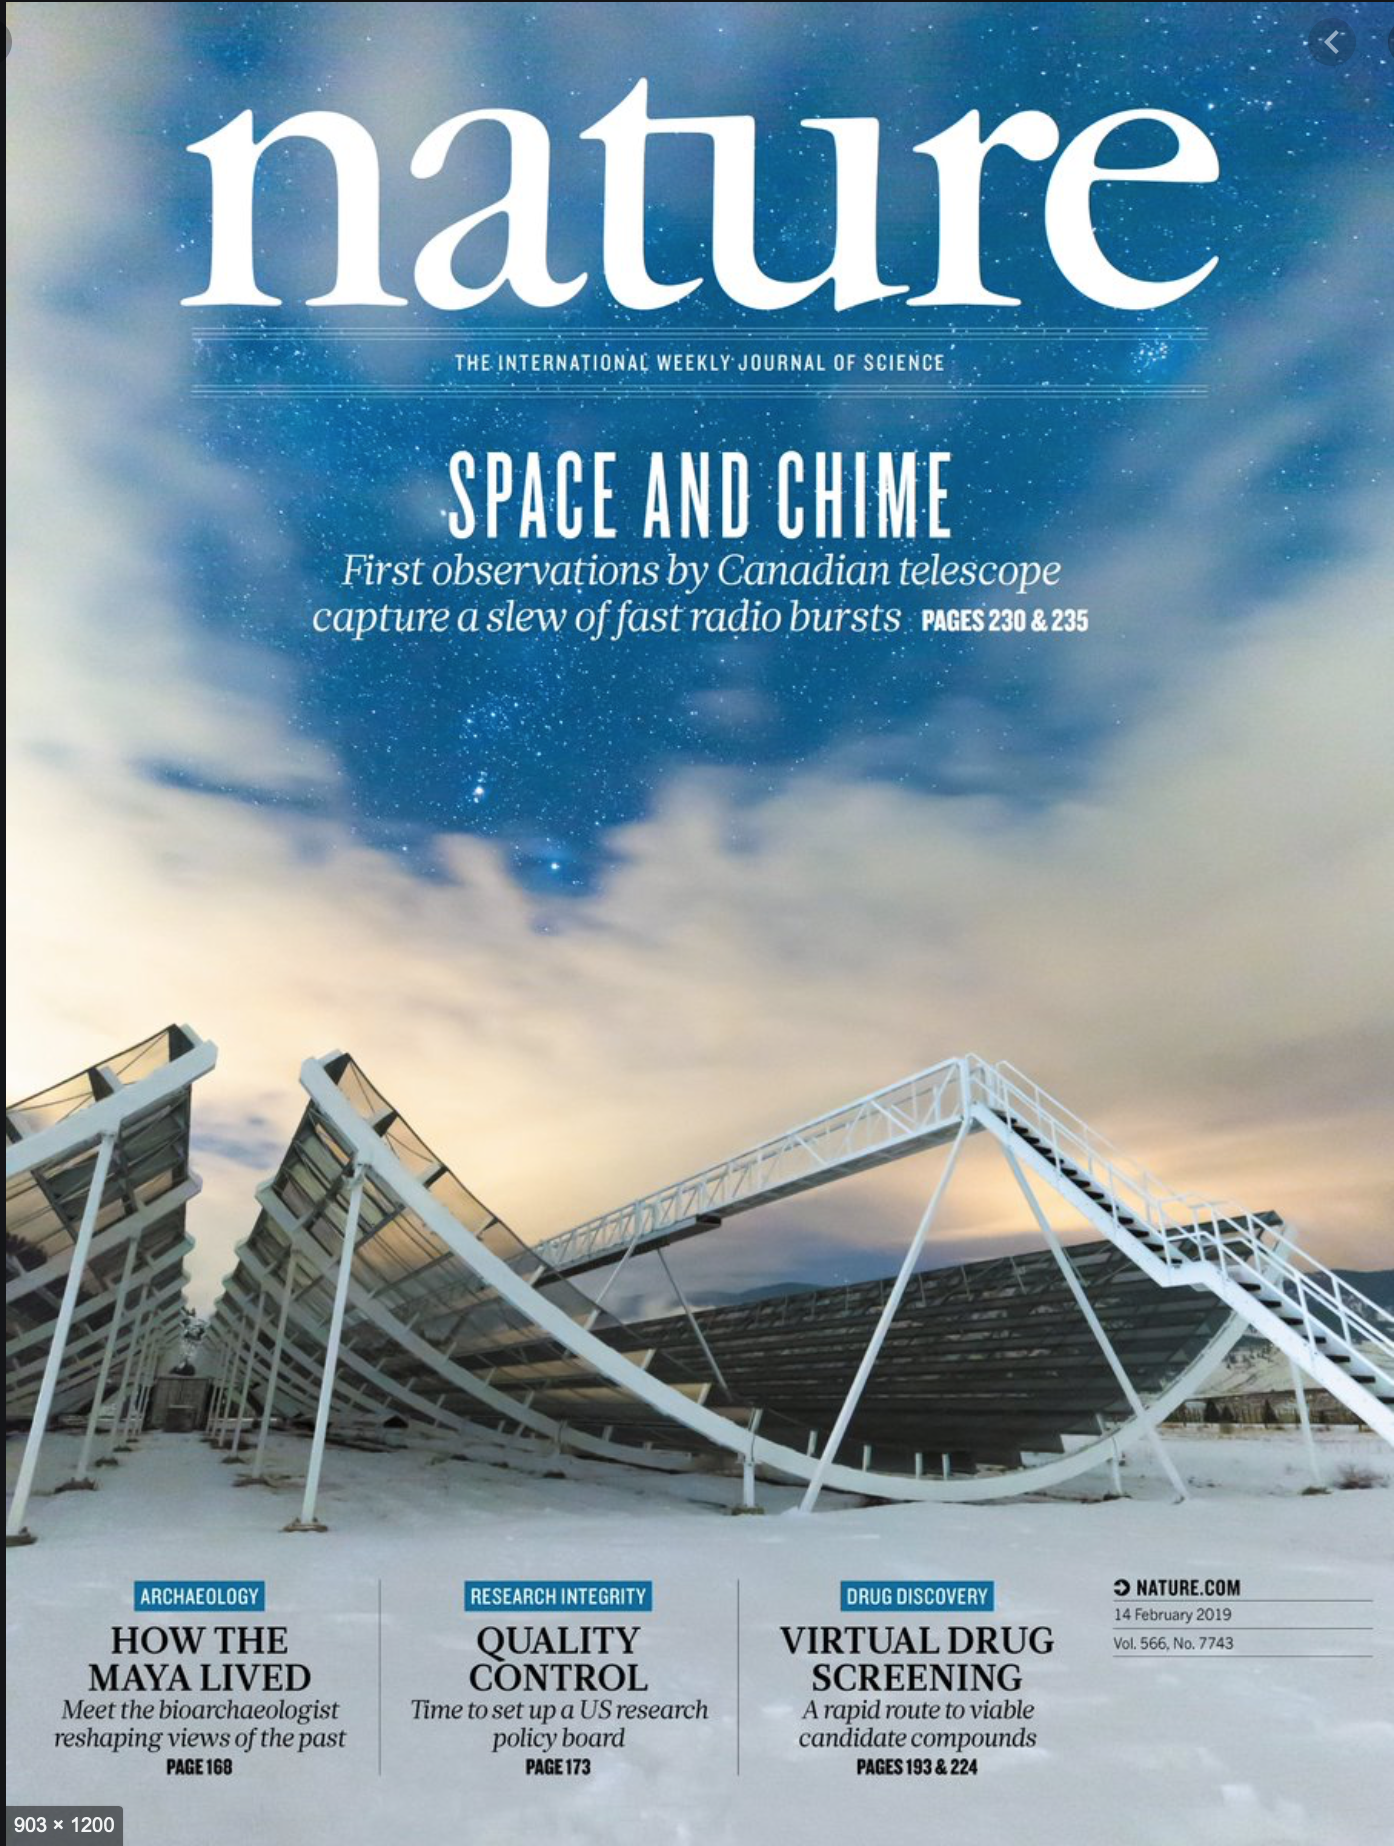
\includegraphics[width=1.8in]{Figures/chime-nature.png}
%\vspace{-0.5in}

}

  \frame{
    \frametitle{Some Recent Results}
    \begin{itemize}
    \item CHIME collaboration 2019, series of FRB papers
    \item event Horizon Telescope, series of papers
    \item Yang, Nishizawa, Pen 2017, ``Testing Gravity with
          Pulsar Scintillation Measurements'', PRD, 95, 4049
        \item Main et al, 2018,``Pulsar emission amplified and resolved by plasma lensing in an eclipsing binary'', Nature, 557, 522
    \end{itemize}
%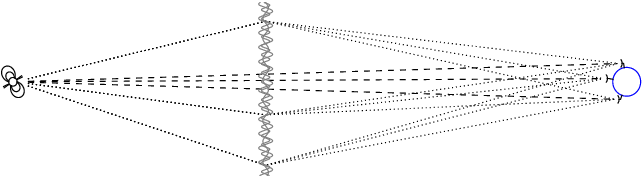
\includegraphics[width=4.5in]{Figures/scintillometry.png}
}

\end{document}
